%===========================================================
%============ Good Thoughts, Good Words, Good Deeds ============
%===========================================================
% Project:      The optimization of Blockchain application in the supply chain finance system using the Particle Swarm optimization algorithm
% Author:       Mahdi Jahangiri
% GitHub:       https://github.com/MahdiJahangiry
% Description:  A professional Beamer template compatible with Persian (XePersian)
%               Includes custom TikZ boxes, progress bars, and optimized layouts.
% ==============================================================================


% ==============================================================================
% 1. DOCUMENT CLASS & PREAMBLE SETUP
% ==============================================================================
\PassOptionsToPackage{x11names, table}{xcolor}
\documentclass[10pt, aspectratio=169, xcolor=dvipsnames, professionalfonts]{beamer}

\mode<presentation>

% !!! CRITICAL SETTING !!!
% Fixes the "Ghost Item" bug in XeTeX/Beamer where hidden items remain visible.
% Sets covered items to be completely invisible instead of transparent.
\setbeamercovered{invisible}


% ==============================================================================
% 2. PERSONAL INFORMATION (Replace with your personal information.)
% ==============================================================================
\newcommand{\MyName}{Mahdi Jahangiri}
\newcommand{\MyPhone}{+98 936 555 8992}
\newcommand{\MyTel}{Mahdi\_Jahangiri7}
\newcommand{\MyEmail}{mehdijh293@gmail.com}
\newcommand{\MyGitHub}{https://github.com/MahdiJahangiry}


% ==============================================================================
% 3. PACKAGES & FONTS
% ==============================================================================
\usepackage[T1]{fontenc}
\usepackage{lmodern}
\usepackage{tikz}
\usepackage{capt-of}
\usepackage{fontawesome5} % For icons like Telegram, GitHub, etc.
\usepackage{dirtree}      % For directory tree visualization
\usepackage{amsmath, amssymb}
\usepackage{graphicx}
\usepackage{booktabs, makecell, multirow, multicol, array}
\usepackage{float}
\usepackage{ragged2e, ulem}
\usepackage{fancyvrb}
\usepackage[ruled,vlined]{algorithm2e} % For algorithms
\usepackage{listings}     % For code listings

% TikZ Libraries
\usetikzlibrary{shadows, positioning, fit, backgrounds, shapes, arrows.meta, calc, decorations.pathreplacing}
\usetikzlibrary{shapes.geometric, shadows.blur}

% Color Definitions
\definecolor{azure4}{RGB}{131,139,139}
\definecolor{maingreen}{RGB}{0, 150, 0} 
\definecolor{deepblue}{RGB}{0, 50, 100} 
\definecolor{me}{rgb}{2.04,0.52,0.1} % Orange accent color

\definecolor{rowgray}{gray}{0.93} 
\definecolor{processblue}{RGB}{230,240,250}
\definecolor{decisiongray}{RGB}{245,245,245}
\definecolor{startgreen}{RGB}{235,245,235}

%Model colors:
\definecolor{layer1color}{RGB}{235, 245, 251}
\definecolor{layer2color}{RGB}{254, 249, 231}
\definecolor{layer3color}{RGB}{232, 248, 245}
\definecolor{mainblue}{RGB}{41, 128, 185}
\definecolor{maingreen}{RGB}{39, 174, 96}
\definecolor{mainorange}{RGB}{230, 126, 34}
\definecolor{mainpurple}{RGB}{142, 68, 173}
\definecolor{darkgray}{RGB}{52, 73, 94}

%Caption:
\usepackage[font=small, labelfont={bf, color=red}, justification=centering]{caption}
\usepackage{subcaption}
\captionsetup[lstlisting]{font={footnotesize}}

% ==============================================================================
% 4. THEME & COLOR CONFIGURATION
% ==============================================================================
\usetheme{Madrid} 
\useoutertheme{miniframes} 

% ==============================================================================
% !!! MATH FONT FIX !!!
% ==============================================================================
%\usefonttheme[onlymath]{serif}

% Apply Custom Colors
\usecolortheme[named=deepblue]{structure}
\setbeamercolor{alerted text}{fg=me}
\setbeamercolor*{palette primary}{use=structure,fg=white,bg=deepblue}
\setbeamercolor*{palette secondary}{use=structure,fg=white,bg=deepblue!75!black}

% Fix Header Colors (Text: Deep Blue, Background: Orange)
\setbeamercolor*{palette tertiary}{use=structure,fg=deepblue,bg=me} 
\setbeamercolor{section in head/foot}{fg=black, bg=me}


% ==============================================================================
% 5. CUSTOM FOOTER (FOOTLINE) DESIGN
% ==============================================================================
% Removes default navigation symbols
\setbeamertemplate{navigation symbols}{}

% Define a physical box for the footer to prevent rendering glitches
\setbeamertemplate{footline}{%
	\leavevmode%
	\hbox{%
		\begin{tikzpicture}
			\useasboundingbox (0,0) rectangle (\paperwidth, 10pt);
			
			% --- Progress Bar (Green) ---
			\ifnum\inserttotalframenumber>0
			\pgfmathsetmacro{\progresswidth}{(\insertframenumber/\inserttotalframenumber)*\paperwidth}
			\fill[maingreen] (0,0) rectangle (\progresswidth pt, 4pt);
			\fi
			
			% --- Info Boxes ---
			% Author Name
			\node[anchor=south west, inner sep=0pt, minimum height=2.5ex, minimum width=0.333\paperwidth, fill=deepblue, text=white, font=\tiny\bfseries] 
			at (0, 4pt) {\hspace{1em}\insertshortauthor};
			
			% Title
			\node[anchor=south west, inner sep=0pt, minimum height=2.5ex, minimum width=0.334\paperwidth, fill=deepblue!75!black, text=white, font=\tiny\bfseries] 
			at (0.333\paperwidth, 4pt) {\centering \insertshorttitle};
			
			% Page Number
			\node[anchor=south west, inner sep=0pt, minimum height=2.5ex, minimum width=0.333\paperwidth, fill=me, text=white, font=\tiny\bfseries] 
			at (0.667\paperwidth, 4pt) {\centering \insertframenumber{} / \inserttotalframenumber};
		\end{tikzpicture}%
	}%
	\vskip0pt%
}


% ==============================================================================
% 6. TIKZ GRAPHIC STYLES
% ==============================================================================
\tikzset{
	basicbox/.style={rectangle, rounded corners=3pt, text width=3.0cm, minimum height=1.3cm, align=center, font=\footnotesize\bfseries, draw=darkgray!50, line width=1pt},
	entitybox/.style={basicbox, top color=white, bottom color=layer1color!80!mainblue, text=darkgray},
	fibox/.style={basicbox, text width=5.0cm, minimum height=1.5cm, top color=white, bottom color=mainblue!30, draw=mainblue, line width=1.5pt, font=\small\bfseries},
	groupbox/.style={basicbox, top color=white, bottom color=layer2color!80!mainorange, text=darkgray, font=\scriptsize\bfseries},
	criteria/.style={rectangle, rounded corners, draw=mainorange!80, fill=white, dashed, font=\scriptsize, align=center, text width=2.5cm},
	engine/.style={rectangle, rounded corners=15pt, minimum width=12.0cm, minimum height=5.0cm, draw=mainpurple, line width=2pt, top color=white, bottom color=mainpurple!15, align=center},
	objective/.style={circle, draw=darkgray, line width=1pt, minimum size=2.1cm, font=\tiny\bfseries, align=center, fill=white, blur shadow, text width=1.6cm},
	db/.style={cylinder, shape border rotate=90, aspect=0.25, draw=maingreen, line width=1.5pt, top color=white, bottom color=maingreen!30, minimum width=2.2cm, minimum height=2.8cm, align=center, font=\scriptsize},
	finalbox/.style={basicbox, draw=maingreen!80!black, top color=white, bottom color=maingreen!40, font=\scriptsize\bfseries},
	arrow/.style={-{Latex[length=3mm, width=2mm]}, line width=1.2pt, draw=darkgray!80},
	bigarrow/.style={-{Latex[length=4mm, width=3mm]}, line width=2pt, draw=mainblue!60},
	dashed_container/.style={rectangle, draw=blue!80, dashed, line width=0.25pt, rounded corners=5pt, inner sep=5pt},
	layer_bg/.style={rounded corners=15pt, line width=1.5pt, inner sep=10pt},
	input_label/.style={font=\scriptsize\bfseries, fill=white, inner sep=3pt, rounded corners, line width=0.8pt}
}

\pgfdeclarelayer{background}
\pgfsetlayers{background,main}


% ==============================================================================
% 7. TCOLORBOX CONFIGURATION (CUSTOM BOXES)
% ==============================================================================
\usepackage{tcolorbox}
\tcbuselibrary{most} 

% --- Global Box Style ---
% Note: 'enhanced' mode is disabled (using 'standard') to prevent 
% rendering artifacts and "ghost items" in XeTeX animations.
\tcbset{
	myboxstyle/.style={
		standard,          
		boxrule=0.5mm,
		fonttitle=\bfseries,
		fontupper=\normalfont,
		separator sign dash,
	}
}

% --- Defined Environments ---
\newtcolorbox{defn}[2]{myboxstyle, colframe=blue!70!black, colback=blue!5, colbacktitle=blue!80!black, title={تعریف: #1}}
\newtcolorbox{ex}[2]{myboxstyle, colframe=green!60!black, colback=green!5, colbacktitle=green!70!black, title={مثال: #1}}
\newtcolorbox{cor}[2]{myboxstyle, colframe=orange!80!black, colback=orange!5, colbacktitle=orange!90!black, title={نتیجه: #1}}
\newtcolorbox{cbl}[2]{myboxstyle, colframe=gray!80!black, colback=gray!5, colbacktitle=gray!90!black, fontupper=\ttfamily, title={قطعه کد: #1}}
\newtcolorbox{objs}[2]{myboxstyle, colframe=violet!70!black, colback=violet!5, colbacktitle=violet!80!black, title={توابع هدف: #1}}
\newtcolorbox{consts}[2]{myboxstyle, colframe=red!70!black, colback=red!5, colbacktitle=red!80!black, title={محدودیت‌ها: #1}}
\newtcolorbox{modell}[2]{myboxstyle, colframe=teal!70!black, colback=teal!5, colbacktitle=teal!80!black, title={مدل: #1}}
\newtcolorbox{expl}[2]{myboxstyle, colframe=cyan!60!black, colback=cyan!5, colbacktitle=cyan!70!black, title={توضیح: #1}}
\newtcolorbox{purp}[2]{myboxstyle, colframe=azure4, colback=azure4!10, colbacktitle=azure4, title={اهداف: #1}}
\newtcolorbox{ques}[2]{myboxstyle, colframe=yellow!60!black, colback=yellow!10, colbacktitle=yellow!70!black, title={سوال‌ها: #1}}
\newtcolorbox{prop}[2]{myboxstyle, colframe=brown!60!black, colback=brown!5, colbacktitle=brown!70!black, title={فرضیه: #1}}
\newtcolorbox{trans}[2]{myboxstyle, colframe=lightgray!80!black, colback=lightgray!10, colbacktitle=lightgray!90!black, title={شفافیت: #1}}
\newtcolorbox{freq}[2]{myboxstyle, colframe=magenta!70!black, colback=magenta!5, colbacktitle=magenta!80!black, title={ظرفیت پردازشی: #1}}


% ==============================================================================
% 8. EXTRA UTILITIES & BIBLIOGRAPHY
% ==============================================================================
\usepackage{zref-abspage}
\usepackage{zref-perpage}
\zmakeperpage{footnote}

\newcommand{\mathlr}[1]{\text{\lr{#1}}}
\renewcommand{\DTstyle}{\ttfamily\scriptsize}
\newcommand{\FileDesc}[1]{\textcolor{gray}{\textit{\scriptsize $\leftarrow$ #1}}}

% Listings Style
\lstdefinestyle{professional_style}{
	backgroundcolor=\color{backcolour},
	commentstyle=\color{codegreen},
	keywordstyle=\color{blue}\bfseries,
	numberstyle=\tiny\color{codegray}\ttfamily,
	stringstyle=\color{codepurple},
	basicstyle=\ttfamily\scriptsize,
	breakatwhitespace=false,
	breaklines=true,
	captionpos=b,
	keepspaces=true,
	numbers=left,
	numbersep=10pt,
	showspaces=false,
	showstringspaces=false,
	showtabs=false,
	tabsize=1,
	frame=lines,
	rulecolor=\color{black},
	framesep=5pt,
	xleftmargin=5pt,
	xrightmargin=5pt,
	aboveskip=10pt,
	belowskip=5pt
}
\lstset{style=professional_style}

% Bibliography Setup (Customizing citation appearance)
\usepackage[nonamebreak, round]{natbib}
\newcommand{\customcite}[1]{%
	\citeauthor{#1}\footnotemark، \citeyear{#1}%
	\LTRfootnotetext{\citeauthor*{#1}}%
}

\makeatletter
\newcounter{mybibcount}
\let\oldbibitem\bibitem
\let\oldthebibliography\thebibliography
\renewcommand{\thebibliography}[1]{%
	\oldthebibliography{#1}%
	\setlength{\leftmargin}{3.5em}
	\setlength{\itemindent}{0pt}
}
\renewcommand{\bibitem}[2][]{%
	\stepcounter{mybibcount}%
	\oldbibitem[#1]{#2}%
	\hspace*{-0.2em}%
	\makebox[1.5em][l]{\textcolor{blue!60!black}{\textbf{\themybibcount.}}}%
	\hspace{0.5em}%
}
\makeatother

% ==============================================================================
% 8.5. MATH FONTS CONFIGURATION (FIXED FOR MAC)
% ==============================================================================
\usepackage{unicode-math} 
\setmathfont{latinmodern-math.otf}

% ==============================================================================
% 8.6. FIX BROKEN SYMBOLS (Checkmark Fix)
% ==============================================================================
\def\checkmark{\tikz\fill[scale=0.4, color=maingreen](0,.35) -- (.25,0) -- (1,.7) -- (.25,.15) -- cycle;}

%%%%%%% Change beamer header font size:
\setbeamerfont{subsection in head/foot}{size=\footnotesize} 

\setbeamerfont{section in head/foot}{size=\tiny, series=\bfseries}



% ==============================================================================
% 9. LANGUAGE SETUP (XEPERSIA)
% ==============================================================================
% Should be loaded last
\usepackage{xepersian}
\settextfont{XB Zar}
\setlatintextfont[Scale=1, AutoFakeSlant=0.2, AutoFakeBold=1.5]{Times New Roman}

% ==============================================================================
% 10. TITLE PAGE
% ==============================================================================
% Fix: Used \texorpdfstring to avoid PDF string warnings
\author[نام شما]{
	\texorpdfstring{\textbf{نام شما}}{Student Name}
	\inst{1}
	\and
	\textbf{نام استاد راهنما}
	\inst{2}
	\vspace{0.3cm}
}

\title[\lr{Thesis Title}]{
	\texorpdfstring{\textbf{\footnotesize \color{white} عنوان پایان‌نامه یا سمینار شما در این قسمت قرار می‌گیرد}}{عنوان}
}

\institute[نام دانشگاه]{\inst{1}دانشکده ...
	\and
	\inst{2} گروه آموزشی ...
	\\\vspace{0.7cm}
	توضیحات تکمیلی (مقطع تحصیلی و رشته)
	\vspace{0.5cm}
}

\date{\today}
\subject{موضوع}

%===========================================================
% 11. DOCUMENT CONTENT
%===========================================================

\begin{document}
	\frame{\maketitle}
	
	\frame{
		\begin{center}
			{\huge \bf بنام او} ...
		\end{center}
	}
	
	% --- Section 1 ---
	\section*{مقدمه}
	\subsection{کلیات}

	\frame{
		طبق 	\citep{chen_blockchain-driven_2020} ...
		\begin{purp}{اهداف اصلی}{}
			\begin{enumerate}
				\item<1-> 
				لورم ایپسوم متن ساختگی با تولید سادگی نامفهوم از صنعت چاپ.
				\vspace{0.3cm}
				\item<2-> 
				هدف دوم: بهبود عملکرد سیستم‌های پیچیده با استفاده از الگوریتم‌های نوین.
				\vspace{0.3cm}
				\item<3-> 
				هدف سوم: کاهش هزینه‌های عملیاتی و افزایش بهره‌وری.
				\item[] 
			\end{enumerate}
		\end{purp}
	}
	
	\frame{
		\begin{ques}{سوالات تحقیق}{}\scriptsize
			\begin{enumerate}
				\item<1-> 
				سوال اول: چگونه می‌توان پارامترهای مدل را بهینه کرد؟
				\vspace{0.3cm}
				\item<2->
				سوال دوم: تاثیر متغیرهای محیطی بر عملکرد سیستم چیست؟
				\vspace{0.3cm}
				\item<3->
				سوال سوم: آیا روش پیشنهادی نسبت به روش‌های سنتی برتری دارد؟
				\item[]
			\end{enumerate}
		\end{ques}
	}
	
	% --- Section 2 ---
	\section{مبانی نظری}
	\subsection{پیشینه تحقیق}
	\frame{
		\begin{table}[htbp]
			\centering
			\caption{جدول مقایسه‌ای پیشینه پژوهش}
			\tiny 
			\setlength{\tabcolsep}{1.4pt} 
			\renewcommand{\arraystretch}{2}
			\definecolor{rowgray}{gray}{0.95}
			\rowcolors{5}{rowgray}{white}
			
			\begin{tabular}{>{\cellcolor{white}}c r l c c c c c c}
				\toprule
				\multirow{2}{*}{\rotatebox{90}{ردیف}} &
				\multirow{2}{*}{محققین} &
				\multirow{2}{*}{حوزه پژوهش} &
				\multirow{2}{*}{رویکرد} &
				\multicolumn{2}{c}{\RL{شاخص‌ها}} &
				\multicolumn{2}{c}{\RL{نوع مدل}} &
				\multirow{2}{*}{پلتفرم} \\
				
				\cmidrule(lr){5-6}
				\cmidrule(lr){7-8}
				
				& & & &
				دقت & سرعت &
				خطی & غیرخطی &
				\\
				
				\midrule
				۱ & \lr{Author A} & موضوع اول & \lr{Method X} & $\checkmark$ &  & $\checkmark$ &  & \lr{MATLAB} \\
				۲ & \lr{Author B} & موضوع دوم & \lr{Method Y} & $\checkmark$ & $\checkmark$ &  & $\checkmark$ & \lr{Python} \\
				۳ & \lr{Author C} & موضوع سوم & \lr{Method Z} &  & $\checkmark$ & $\checkmark$ &  & \lr{Java} \\
				۴ & \textbf{این پژوهش} & \textbf{روش پیشنهادی} & \textbf{\lr{Proposed}} & \textbf{$\checkmark$} & \textbf{$\checkmark$} &  & \textbf{$\checkmark$} & \textbf{\lr{C++}} \\
				\bottomrule
			\end{tabular}
		\end{table}
	}
	
	% --- Section 3 ---
	\section{روش‌شناسی}
	

	\subsection{تعاریف و پارامترهای مدل}
	\frame{
		\begin{table}[H]
			\centering
			\label{tab:generic_parameters}
			\tiny % سایز فونت ریز
			\fontsize{4.2}{6}\selectfont
			\setlength{\tabcolsep}{0.3pt} 
			\renewcommand{\arraystretch}{1.2} % فاصله خطوط را کمی بیشتر کردم چون تعداد سطرها کم شده
			
			\definecolor{rowgray}{gray}{0.95}
			\rowcolors{2}{rowgray}{white}
			
			\begin{tabular}{c p{8cm}}
				\toprule
				\textbf{نماد} & \textbf{تعریف و توضیح} \\
				\midrule
				
				$i$ & شاخص مجموعه اول لورم ایپسوم، $i = 1, \ldots, I$ \\
				
				$j$ & شاخص مجموعه دوم متن ساختگی، $j = 1, \ldots, J$ \\
				
				$k$ & شاخص سناریوهای مختلف در بازه زمانی مشخص \\
				
				$C_{ij}^{fix}$ & پارامتر هزینه ثابت برای تخصیص منابع در حالت $i$ و $j$ \\
				
				$C_{ij}^{var}$ & پارامتر هزینه متغیر مرتبط با پردازش داده‌های ساختگی \\
				
				$T_{max}$ & حداکثر زمان مجاز برای تکمیل فرآیند لورم ایپسوم \\
				
				$\alpha_{i}$ & ضریب اهمیت یا وزن‌دهی به شاخص $i$ در تابع هدف \\
				
				$\beta_{j}$ & پارامتر تنظیم‌کننده حساسیت مدل نسبت به تغییرات \\
				
				$X_{ij}$ & متغیر تصمیم‌گیری باینری؛ اگر گزینه $i$ به $j$ تخصیص یابد برابر ۱، در غیر این صورت ۰ \\
				
				$Y_{k}$ & متغیر پیوسته نشان‌دهنده مقدار جریان در سناریوی $k$ \\
				
				\bottomrule
			\end{tabular}
		\end{table}
	}
	
	\subsection{فرمولاسیون مسئله}
	\frame{
		\begin{objs}{توابع هدف (نمونه)}{}\scriptsize
			\uncover<1->{
				\begin{equation}
					\mathbf{Z_1} = \min \sum_{i=1}^{N} \left( \alpha \cdot x_i^2 + \beta \cdot y_i \right)
				\end{equation}\vspace{-0.5cm}
			}
			\uncover<2->{
				\begin{equation}
					\mathbf{Z_2} = \max \int_{0}^{T} f(t) \, dt
				\end{equation}\vspace{-0.5cm}
			}
			\uncover<3->{
				\begin{equation}
					\mathbf{Z_3} = \frac{\partial E}{\partial w} \approx \Delta w \cdot \eta
				\end{equation}
			}
		\end{objs}
	}
	
	\frame{
		\begin{consts}{محدودیت‌ها (نمونه)}{}\scriptsize
			\uncover<1->{
				\begin{equation}
					\sum_{j=1}^{M} x_{ij} \le C_{max}, \quad \forall i
				\end{equation}\vspace{-0.5cm}
			}
			\uncover<2->{
				\begin{equation}
					x_{ij} \in \{0, 1\} \quad \text{(Binary Constraint)}
				\end{equation}
			}
		\end{consts}
	}
	

	
	% --- Section 4 ---
	\section{نتایج}
	\subsection{ارزیابی عملکرد}
	
	% Example of Complex Visual Table
	\begin{frame}
		\begin{figure}[ht]
			\centering
			\resizebox{!}{0.85\textheight}{%
				\begin{tikzpicture}[
					scale=1, 
					transform shape,
					node distance=0.6cm and 0.5cm, 
					groupNodeOrg/.style={rectangle, draw=blue!70!black, top color=blue!5, bottom color=blue!15, rounded corners=6pt, minimum height=0.8cm, minimum width=3.2cm, align=center, font=\small\bfseries},
					groupNodeInd/.style={rectangle, draw=teal!70!black, top color=teal!5, bottom color=teal!15, rounded corners=6pt, minimum height=0.8cm, minimum width=3.2cm, align=center, font=\small\bfseries},
					schemeNode/.style={rectangle, draw=gray!40, fill=white, rounded corners=3pt, minimum height=0.6cm, minimum width=2.2cm, align=center, font=\footnotesize, anchor=west},
					selectedNode/.style={rectangle, draw=green!60!black, top color=green!5, bottom color=green!20, line width=1.5pt, rounded corners=3pt, minimum height=0.6cm, minimum width=2.2cm, align=center, font=\footnotesize\bfseries, anchor=west},
					checkBadge/.style={circle, fill=green!60!black, text=white, inner sep=1pt, scale=0.7, anchor=north east}
					]
					% Vector Display Node
					\node[rectangle, draw=black, thick, fill=yellow!10, rounded corners=5pt, minimum width=8cm, minimum height=0.8cm, font=\large\bfseries] (vector) at (0, 0) {$\vec{X} = [A, B, A, C, B, A]$};
					
					% Group 1
					\node[groupNodeOrg, below=0.6cm of vector.south west, anchor=north west, xshift=0.5cm] (g11) {\faBuilding\ \rl{دسته اول - سطح ۱}};
					\node[schemeNode, right=0.5cm of g11.east] (s11_1) {\lr{Option 1}};
					\node[selectedNode, right=0.2cm of s11_1] (s11_2) {\lr{Option 2}};
					\node[checkBadge] at (s11_2.north east) {\checkmark};
					\node[schemeNode, right=0.2cm of s11_2] (s11_3) {\lr{Option 3}};
					
					% Group 2
					\node[groupNodeOrg, below=0.4cm of g11] (g12) {\faBuilding\ \rl{دسته اول - سطح ۲}};
					\node[schemeNode] at (s11_1.west |- g12) (s12_1) {\lr{Option 1}};
					\node[schemeNode] at (s11_2.west |- g12) (s12_2) {\lr{Option 2}};
					\node[selectedNode] at (s11_3.west |- g12) (s12_3) {\lr{Option 3}};
					\node[checkBadge] at (s12_3.north east) {\checkmark};
					
					% Group 3
					\node[groupNodeInd, below=0.8cm of g12] (g21) {\faUser\ \rl{دسته دوم - سطح ۱}};
					\node[selectedNode] at (s11_1.west |- g21) (s21_1) {\lr{Option 1}};
					\node[checkBadge] at (s21_1.north east) {\checkmark};
					\node[schemeNode] at (s11_2.west |- g21) (s21_2) {\lr{Option 2}};
					\node[schemeNode] at (s11_3.west |- g21) (s21_3) {\lr{Option 3}};
					
					% Decoration
					\draw [decorate,decoration={brace,amplitude=6pt,mirror=false}, thick, color=green!60!black]
					([yshift=5pt]s11_1.north west) -- ([yshift=5pt]s11_3.north east) 
					node [green!60!black,midway,yshift=15pt, font=\scriptsize\bfseries] {\rl{گزینه‌های موجود}};
					
					% Background Layer
					\begin{pgfonlayer}{background}
						\coordinate (box_left) at ([xshift=-1.0cm]g11.west); 
						\coordinate (box_right) at ([xshift=0.2cm]g11.east);
						\node[fit=(g11)(g12)(g11-|box_left)(g11-|box_right), fill=blue!5, draw=blue!20, rounded corners=10pt, dashed, thick, inner sep=5pt] {};
					\end{pgfonlayer}
			\end{tikzpicture}}
			\caption{نمونه بصری‌سازی گرافیکی انتخاب‌ها}
		\end{figure}
	\end{frame}
	
	% --- Section 5 ---
	\section{نتیجه‌گیری}
	\subsection{دستاوردهای کلیدی}
	\frame{
		\begin{tikzpicture}[remember picture, overlay]
			\tikzset{
				card/.style={rectangle, rounded corners=12pt, minimum width=5.8cm, minimum height=2.7cm, text width=5.2cm, align=center, drop shadow={opacity=0.25}, inner sep=8pt, font=\small},
				icon_circle/.style={circle, fill=white, minimum size=1.0cm, drop shadow={opacity=0.15}}
			}
			
			\onslide<1->{
				\node[card, top color=blue!5, bottom color=white, draw=deepblue!30] (c1) at ([xshift=3.2cm, yshift=1.4cm]current page.center) {
					\vspace{0.4cm} 
					\textbf{\textcolor{deepblue}{\rl{۱. نوآوری اول}}}\\
					\vspace{0.1cm} \scriptsize \color{gray!40!black}
					\rl{توسعه مدل ریاضی جدید با رویکرد بهینه‌سازی چندهدفه.}
				};
				\node[icon_circle] at (c1.north) {\large \textcolor{deepblue}{\faCalculator}};
			}
			
			\onslide<2->{
				\node[card, top color=blue!5, bottom color=white, draw=deepblue!30] (c2) at ([xshift=-3.2cm, yshift=1.4cm]current page.center) {
					\vspace{0.4cm}
					\textbf{\textcolor{deepblue}{\rl{۲. نوآوری دوم}}}\\
					\vspace{0.1cm} \scriptsize \color{gray!40!black}
					\rl{پیاده‌سازی الگوریتم بر روی داده‌های شبیه‌سازی شده.}
				};
				\node[icon_circle] at (c2.north) {\large \textcolor{deepblue}{\faCogs}};
			}
			
			\onslide<3->{
				\node[card, top color=me!10, bottom color=white, draw=me] (c4) at ([xshift=0cm, yshift=-2.0cm]current page.center) {
					\vspace{0.4cm}
					\textbf{\textcolor{me}{\rl{نتیجه نهایی}}}\\
					\vspace{0.1cm} \scriptsize \color{gray!40!black}
					\rl{بهبود کارایی سیستم به میزان قابل توجه و کاهش خطاها.}
				};
				\node[icon_circle, draw=me!50] at (c4.north) {\large \textcolor{me}{\faStar}};
			}
		\end{tikzpicture}
	}
	
	
	
	\subsection{پاسخ به سوالات پژوهش}
	\frame{
		\begin{tikzpicture}[remember picture, overlay]
			% --- Style Definitions ---
			\tcbset{
				q_box_style/.style={width=0.45\textwidth, enhanced, colframe=gray!40, colback=white, coltitle=darkgray, fonttitle=\bfseries\scriptsize, fontupper=\scriptsize\bfseries, arc=5pt, boxrule=1pt, drop shadow={opacity=0.1}, halign=center, valign=center, height=1.2cm},
				popup_style/.style={width=0.85\textwidth, enhanced, colback=white, colframe=deepblue, fonttitle=\bfseries\large, fontupper=\small, arc=8pt, boxrule=1.5pt, drop shadow={opacity=0.5, shadow xshift=2pt, shadow yshift=-2pt}, attach boxed title to top center={yshift=-10pt}, boxed title style={colback=deepblue, frame hidden, arc=5pt}, halign=center, top=12pt, bottom=12pt, left=12pt, right=12pt}
			}
			\tikzstyle{glass_layer}=[fill=white, opacity=0.88, text opacity=1]
			
			% --- Questions Layout (4 Corners) ---
			\onslide<1->{
				\node[anchor=north east] at ([xshift=-0.5cm, yshift=-1.5cm]current page.north east) {
					\begin{tcolorbox}[q_box_style, colframe=deepblue!50] \rl{۱. سوال پژوهشی اول لورم ایپسوم؟} \end{tcolorbox}
				};
			}
			\onslide<3->{
				\node[anchor=north west] at ([xshift=0.5cm, yshift=-1.5cm]current page.north west) {
					\begin{tcolorbox}[q_box_style, colframe=mainorange!50] \rl{۲. سوال پژوهشی دوم لورم ایپسوم؟} \end{tcolorbox}
				};
			}
			\onslide<5->{
				\node[anchor=south east] at ([xshift=-0.5cm, yshift=1.0cm]current page.south east) {
					\begin{tcolorbox}[q_box_style, colframe=mainpurple!50] \rl{۳. سوال پژوهشی سوم لورم ایپسوم؟} \end{tcolorbox}
				};
			}
			\onslide<7->{
				\node[anchor=south west] at ([xshift=0.5cm, yshift=1.0cm]current page.south west) {
					\begin{tcolorbox}[q_box_style, colframe=maingreen!50] \rl{۴. سوال پژوهشی چهارم لورم ایپسوم؟} \end{tcolorbox}
				};
			}
			
			% --- Answers Popups (Overlays) ---
			
			% Answer 1
			\only<2>{
				\fill[glass_layer] (current page.south west) rectangle (current page.north east);
				\node at (current page.center) {
					\begin{tcolorbox}[popup_style, title={\rl{پاسخ ۱: عنوان پاسخ لورم ایپسوم}}, colframe=deepblue, boxed title style={colback=deepblue}]
						\faUniversity \ \textbf{\rl{تیتر اصلی پاسخ اول}}
						\par \vspace{0.3cm}
						\rl{لورم ایپسوم متن ساختگی با تولید سادگی نامفهوم از صنعت چاپ و با استفاده از طراحان گرافیک است. چاپگرها و متون بلکه روزنامه و مجله در ستون و سطرآنچنان که لازم است.}
					\end{tcolorbox}
				};
			}
			
			% Answer 2
			\only<4>{
				\fill[glass_layer] (current page.south west) rectangle (current page.north east);
				\node at (current page.center) {
					\begin{tcolorbox}[popup_style, title={\rl{پاسخ ۲: عنوان پاسخ لورم ایپسوم}}, colframe=mainorange, boxed title style={colback=mainorange}]
						\faChartLine \ \textbf{\rl{تیتر اصلی پاسخ دوم}}
						\par \vspace{0.3cm}
						\rl{لورم ایپسوم متن ساختگی با تولید سادگی نامفهوم از صنعت چاپ و با استفاده از طراحان گرافیک است. چاپگرها و متون بلکه روزنامه و مجله در ستون و سطرآنچنان که لازم است.}
					\end{tcolorbox}
				};
			}
			
			% Answer 3
			\only<6>{
				\fill[glass_layer] (current page.south west) rectangle (current page.north east);
				\node at (current page.center) {
					\begin{tcolorbox}[popup_style, title={\rl{پاسخ ۳: عنوان پاسخ لورم ایپسوم}}, colframe=mainpurple, boxed title style={colback=mainpurple}]
						\faLayerGroup \ \textbf{\rl{تیتر اصلی پاسخ سوم}}
						\par \vspace{0.3cm}
						\rl{لورم ایپسوم متن ساختگی با تولید سادگی نامفهوم از صنعت چاپ و با استفاده از طراحان گرافیک است. چاپگرها و متون بلکه روزنامه و مجله در ستون و سطرآنچنان که لازم است.}
					\end{tcolorbox}
				};
			}
			
			% Answer 4
			\only<8>{
				\fill[glass_layer] (current page.south west) rectangle (current page.north east);
				\node at (current page.center) {
					\begin{tcolorbox}[popup_style, title={\rl{پاسخ ۴: عنوان پاسخ لورم ایپسوم}}, colframe=maingreen, boxed title style={colback=maingreen}]
						\faRocket \ \textbf{\rl{تیتر اصلی پاسخ چهارم}}
						\par \vspace{0.3cm}
						\rl{لورم ایپسوم متن ساختگی با تولید سادگی نامفهوم از صنعت چاپ و با استفاده از طراحان گرافیک است. چاپگرها و متون بلکه روزنامه و مجله در ستون و سطرآنچنان که لازم است.}
					\end{tcolorbox}
				};
			}
		\end{tikzpicture}
	}
	
	
	% --- Roadmap ---
	\frame{
		\begin{tikzpicture}[remember picture, overlay]
			\tikzset{
				milestone/.style={circle, fill=white, draw=deepblue, line width=2pt, minimum size=1.3cm, drop shadow={opacity=0.25}, font=\Large},
				info_card/.style={rectangle, rounded corners=8pt, fill=white, draw=gray!30, line width=1pt, text width=3.4cm, align=center, font=\scriptsize, inner sep=5pt, drop shadow={opacity=0.15}, anchor=north},
				time_label/.style={font=\bfseries\small\color{deepblue}, yshift=0.4cm},
				path_line/.style={draw=gray!30, line width=3pt, rounded corners=20pt, dashed}
			}
			
			\node[anchor=north] at ([yshift=-1.5cm]current page.north) {
				\large \textbf{\textcolor{deepblue}{\rl{نقشه راه آینده}}}
			};
			\coordinate (center_y) at ([yshift=-0.5cm]current page.center);
			\coordinate (start) at ([xshift=4.5cm]center_y); 
			\coordinate (mid)   at (center_y);
			\coordinate (end)   at ([xshift=-4.5cm]center_y); 
			
			\onslide<1->{ \draw[path_line] (start) -- (mid) -- (end); }
			
			\onslide<2->{
				\node[milestone, draw=maingreen] (m1) at (start) {\textcolor{maingreen}{\faQuestionCircle}};
				\node[time_label] at (m1.north) {\rl{فاز اول}};
				\node[info_card, top color=green!5, bottom color=white] at ([yshift=-0.4cm]m1.south) {
					\textbf{\textcolor{maingreen!60!black}{\rl{بررسی اولیه}}}\\ \vspace{0.1cm} \color{gray!40!black} \rl{مطالعات امکان‌سنجی.}
				};
			}
			\onslide<3->{
				\node[milestone, draw=mainorange] (m2) at (mid) {\textcolor{mainorange}{\faBrain}};
				\node[time_label] at (m2.north) {\rl{فاز دوم}};
				\node[info_card, top color=orange!5, bottom color=white] at ([yshift=-0.4cm]m2.south) {
					\textbf{\textcolor{mainorange!80!black}{\rl{هوش مصنوعی}}}\\ \vspace{0.1cm} \color{gray!40!black} \rl{افزودن یادگیری ماشین.}
				};
			}
			\onslide<4->{
				\node[milestone, draw=mainpurple] (m3) at (end) {\textcolor{mainpurple}{\faGlobe}};
				\node[time_label] at (m3.north) {\rl{فاز سوم}};
				\node[info_card, top color=violet!5, bottom color=white] at ([yshift=-0.4cm]m3.south) {
					\textbf{\textcolor{mainpurple!80!black}{\rl{گسترش}}}\\ \vspace{0.1cm} \color{gray!40!black} \rl{پیاده‌سازی در مقیاس جهانی.}
				};
			}
		\end{tikzpicture}
	}
	
	
\section{مرور کلی}
	
	
	\frame{
		\begin{tikzpicture}[remember picture, overlay]
			\tikzset{
				core_node/.style={rectangle, rounded corners=6pt, minimum width=2.8cm, minimum height=1.4cm, text width=2.6cm, align=center, drop shadow={opacity=0.15}, font=\scriptsize\bfseries, inner sep=3pt},
				step_circle/.style={circle, fill=white, draw=deepblue, line width=1.2pt, minimum size=0.6cm, font=\bfseries\scriptsize, drop shadow},
				tag_node/.style={rectangle, rounded corners=4pt, fill=white, draw=red!70, dashed, line width=0.8pt, font=\tiny\bfseries, inner sep=3pt, text=gray!60!black, align=center, drop shadow={opacity=0.05}},
				tag_line/.style={draw=gray!30, line width=0.8pt},
				flow_line/.style={draw=gray!20, line width=4pt, rounded corners=20pt, ->, >=Latex}
			}
			
			\node[anchor=north] at ([yshift=-1.5cm]current page.north) {
				\large \textbf{\textcolor{deepblue}{\rl{عنوان کلی دیاگرام لورم ایپسوم}}}
			};
			\coordinate (c1) at ([xshift=-5.5cm, yshift=0.5cm]current page.center); 
			\coordinate (c2) at ([xshift=-2.8cm, yshift=-1.8cm]current page.center); 
			\coordinate (c3) at ([xshift=0cm, yshift=0.5cm]current page.center);    
			\coordinate (c4) at ([xshift=2.8cm, yshift=-1.8cm]current page.center);  
			\coordinate (c5) at ([xshift=5.5cm, yshift=0.5cm]current page.center);   
			
			\onslide<1->{ \draw[flow_line] (c1) -- (c2) -- (c3) -- (c4) -- (c5); }
			
			\onslide<1->{
				\node[core_node, top color=red!5, bottom color=white, draw=red!40] (n1) at (c1) { \textcolor{red!70!black}{\faExclamationTriangle}\\ \vspace{0.05cm} \rl{مرحله اول} };
				\node[step_circle, draw=red!60] at ([yshift=0.35cm]n1.north) {1};
				\node[tag_node] (t1a) at ([yshift=1.3cm, xshift=-1.0cm]n1) {Lorem Ipsum 1};
				\node[tag_node] (t1b) at ([yshift=1.3cm, xshift=1.0cm]n1) {Lorem Ipsum 2};
				\node[tag_node] (t1c) at ([yshift=-1.3cm]n1) {Lorem Ipsum 3};
				\draw[tag_line] (n1) -- (t1a); \draw[tag_line] (n1) -- (t1b); \draw[tag_line] (n1) -- (t1c);
			}
			
			\onslide<2->{
				\node[core_node, top color=blue!5, bottom color=white, draw=blue!40] (n2) at (c2) { \textcolor{blue!70!black}{\faCalculator}\\ \vspace{0.05cm} \rl{مرحله دوم} };
				\node[step_circle, draw=blue!60] at ([yshift=-0.35cm]n2.south) {2};
				\node[tag_node] (t2a) at ([yshift=1.3cm]n2) {Lorem Ipsum 4};
				\node[tag_node] (t2b) at ([yshift=-1.3cm, xshift=-1.0cm]n2) {Lorem Ipsum 5};
				\node[tag_node] (t2c) at ([yshift=-1.3cm, xshift=1.0cm]n2) {Lorem Ipsum 6};
				\draw[tag_line] (n2) -- (t2a); \draw[tag_line] (n2) -- (t2b); \draw[tag_line] (n2) -- (t2c);
			}
			
			\onslide<3->{
				\node[core_node, top color=violet!5, bottom color=white, draw=violet!40] (n3) at (c3) { \textcolor{violet!70!black}{\faCogs}\\ \vspace{0.05cm} \rl{مرحله سوم} };
				\node[step_circle, draw=violet!60] at ([yshift=0.35cm]n3.north) {3};
				\node[tag_node] (t3a) at ([yshift=1.3cm, xshift=-1.2cm]n3) {Lorem Ipsum 7};
				\node[tag_node] (t3b) at ([yshift=1.3cm, xshift=1.2cm]n3) {Lorem Ipsum 8};
				\node[tag_node] (t3c) at ([yshift=-1.3cm, xshift=-1.2cm]n3) {Lorem Ipsum 9};
				\node[tag_node] (t3d) at ([yshift=-1.3cm, xshift=1.2cm]n3) {Lorem Ipsum 10};
				\draw[tag_line] (n3) -- (t3a); \draw[tag_line] (n3) -- (t3b); \draw[tag_line] (n3) -- (t3c); \draw[tag_line] (n3) -- (t3d);
			}
			
			\onslide<4->{
				\node[core_node, top color=maingreen!5, bottom color=white, draw=maingreen!40] (n4) at (c4) { \textcolor{maingreen!70!black}{\faChartLine}\\ \vspace{0.05cm} \rl{مرحله چهارم} };
				\node[step_circle, draw=maingreen!60] at ([yshift=-0.35cm]n4.south) {4};
				\node[tag_node] (t4a) at ([yshift=1.3cm]n4) {Lorem Ipsum 11};
				\node[tag_node] (t4b) at ([yshift=-1.3cm, xshift=-1.0cm]n4) {Lorem Ipsum 12};
				\node[tag_node] (t4c) at ([yshift=-1.3cm, xshift=1.0cm]n4) {Lorem Ipsum 13};
				\draw[tag_line] (n4) -- (t4a); \draw[tag_line] (n4) -- (t4b); \draw[tag_line] (n4) -- (t4c);
			}
			
			\onslide<5->{
				\node[core_node, top color=orange!5, bottom color=white, draw=orange!40] (n5) at (c5) { \textcolor{orange!70!black}{\faLightbulb}\\ \vspace{0.05cm} \rl{مرحله پنجم} };
				\node[step_circle, draw=orange!60] at ([yshift=0.35cm]n5.north) {5};
				\node[tag_node] (t5a) at ([yshift=1.3cm, xshift=-1.0cm]n5) {Lorem Ipsum 14};
				\node[tag_node] (t5b) at ([yshift=1.3cm, xshift=1.0cm]n5) {Lorem Ipsum 15};
				\node[tag_node] (t5c) at ([yshift=-1.3cm]n5) {Lorem Ipsum 16};
				\draw[tag_line] (n5) -- (t5a); \draw[tag_line] (n5) -- (t5b); \draw[tag_line] (n5) -- (t5c);
			}
		\end{tikzpicture}
	}
	
	
	% --- Thank You ---

	\frame{
		\begin{latin}
			\begin{center}
				\vspace{0.5cm}
				{\LARGE \bfseries Thank You for Your Attention}
			\end{center}
			\vspace{1cm}
			\begin{columns}
				\begin{column}{0.45\textwidth}
					\uncover<2->{
						\begin{latin}
							\begin{itemize}
								\setlength\itemsep{1.2em} 
								\item[\faFedora] \textbf{\MyName}
								\item[\faTelegramPlane] \MyTel
								\item[\faMailBulk] \MyEmail
								\item[\faGithub] \MyGitHub
							\end{itemize}
						\end{latin}
					}
				\end{column}
				\begin{column}{0.55\textwidth}
					\uncover<3->{
						\begin{latin}
							\centering
							\begin{beamercolorbox}[sep=10pt,center,rounded=true,shadow=true]{palette tertiary}
								\small \itshape
								``Diversity in counsel, unity in command.''
								\par \vspace{0.3cm}
								\tiny \textbf{--- Cyrus the Great}
							\end{beamercolorbox}
							\vspace{0.8cm}
							\footnotesize \color{gray}
							\faHeart \ Proudly dedicated to my homeland, \textbf{Iran}.
						\end{latin}
					}
				\end{column}
			\end{columns}
		\end{latin}
	}
	
	%\section{مراجع}
	\frame{
		\bibliographystyle{asa-fa}
		\bibliography{refb.bib}
	}
\end{document}